\chapter{Integration of Pccf with detectors}

\section{From SDM: Integration of PCCF into a change detector}
\label{sec:pccf_integration}
%\subsection{Integration of an individual change detector with PCCF}
There are two straightforward approaches for using PCCF can be used to potentially improve the accuracy of existing change detectors:
(1)~post-processing -- a detector with fixed settings is used; its output (CDEs) are adjusted based on PCCFs values,
and (2)~pre-processing -- the sensitivity of the detector is dynamically adjusted according to the current PCCFs values.

At the beginning of the change detection process initial probabilities of changes in the foreseeable future are computed using PCCF.
After that PCCF is recalculated every time the last confirmed $c_i$ is known.

In case of post-processing, a change detector with fixed settings, learned offline, is applied.
When the detector alarms a change at time $t$, we check whether the probability of change given by PCCF is greater than a user defined threshold $\mathcal{P}(t) > p_h$.
If it is, we count CDE as a change and output $\Event{t}{+}$, otherwise we output $\Event{t}{-}$.

In case of pre-processing, detector's settings are adjusted dynamically according to PCCF. The detector is made more sensitive when a change is expected with a higher probability $\mathcal{P}(t) > p_h$, and less sensitive when the change is expected with a lower probability.
This strategy should be applied with caution in order not to make the detector too sensitive, which would result in an increase the FP rate.
In this study we consider only scenario when the highest value of the dynamically adjusted sensitivity of the detector is equal to the optimal threshold value learned during the training phase.
When the estimated probability of the change given by PCCF is low, the sensitivity threshold is lowered.
This scenario is illustrated in Figure~\ref{fig:naivedetector} where detector's sensitivity is a function of PCCF.

\subsection{Experiments}
\label{subsec:experiments}
To illustrate the utility of the PCCF we performed three experiments using artificially generated data and two experiments with real data.
\footnote{We have made the code for computing PCCF and running simulations and experiments publicly available at \url{https://github.com/av-maslov/Pccf}.}.
Our goal is to improve the accuracy of online change detection when recurrent changes are expected.
The required information about recurrence is the time intervals between consecutive changes, given as the parameters of the normal distribution $N(\theta = \mu, \sigma)$.
%After the simulation results, we present the fourth part of the experimental study, in which we demonstrate utility of PCCF on two real data sets.

\subsection{PCCF simulation.}
In order to confirm the correctness of the PCCF Eq.~(\ref{eq:pccf_recurren_1}),~(\ref{eq:gaussian_pccf}) expressing the probability to observe a recurrent change at every moment $t$, we performed a simulation by generating sequences of the recurrent changes multiple times and calculating frequencies of occurrence of generated time locations of the changes at each moment of time.
% (see Algorithm~\ref{alg:pccf_sim} in the appendix).
The shape of the obtained curve of frequencies perfectly fits analytically computed PCCF function.

\subsection{Delay of change confirmation.}
In this simulation we illustrate a procedure to estimate maximum delay of change confirmation $D$ during which the recurrence information in a form of parameters $\theta = (\mu, \sigma)$ is still useful and demonstrate the use of PCCF in post-processing settings.

From Figures~\ref{fig:pccf_example} and~\ref{fig:conffunction} depicting behavior of the PCCF it can be seen that the probability of a change oscillates with decreasing amplitude and converges to the limit $L$.
Assuming the probability of making a FP at any moment is constant and is equal to $\lambda$, there are three scenarios to consider:
\begin{enumerate}
\setlength\itemsep{0pt}
\item The error rate $\lambda$ is higher than $\mathcal{P}(t)$ for all $t$.
In this case the detection accuracy cannot be improved with recurrence information $\theta$;
\item $\lambda$ is higher than the limit $L$ but it is lower than the local maximums of the PCCF $\mathcal{P}(t)$. This case is depicted in Figure~\ref{fig:conffunction} by the horizontal dashed line with value $0.2$.
\item $\lambda$ is lower than the limit $L$; this case is depicted with the horizontal dashed line with value $0.05$.
\end{enumerate}
We are not interested in the first case because the probability of making errors is so high that the baseline change detector should be optimized better first.
In the second case peaks of $\mathcal{P}(t)$ at moments $t = i \mu$ are higher than $\lambda$ until some moment $D$ (vertical line), after which the probability of the error is always higher than the probability of change.
The third case is equivalent to the first case till the moment when local minimums of $\mathcal{P}(t)$ become always larger than $\lambda$.
These observations suggest that we can determine the maximum tolerable confirmation delay $D$ (Figure~\ref{fig:conffunction}) by computing the PCCF function, estimating the error rate of detector, and finding the last peak of $\mathcal{P}(t)$ which is higher than $\lambda$.
To confirm our hypothesis we run the following experiment.

\emph{Input data description}.
For each delay $D$ in the range from 5 to 300 we generate input signal $500$ times with $50$ recurrent change points with $\mu = 10$ and $\sigma = 0.7$.
%The average distance  between changes and its standard deviation are set to $(\mu = 10, \sigma = 0.7)$.
PCCF $\mathcal{P}(t | \mu, \sigma)$ is calculated and updated after the location of the last change is output with the current delay value $D$.
Change point locations are generated according to Definition~\ref{def:recurrentdefinition}, i.e.\ given  $c_1$, the second change is $c_2 = c_1 + \epsilon_1$, $c_3 = c_2 + \epsilon_3$ and so on,  where $\epsilon_i$ is a sample from the Gaussian distribution. %of the first change $p(c_1|\theta = \mu, \sigma)$.
The error rate defining the expected number of FPs per $\mu$ is set to $\lambda = (0.05, 0.2)$.
Time locations of outliers are sampled from the uniform distribution so that there are $1/\lambda$ outliers per time interval of width $\mu$ where $\lambda$ is the FP rate of the detector.

\emph{Change detector.}
In this and the next simulation for PCCF pre-processing we used artificially generated data streams, in which changes are abrupt step changes in the value of the signal.
We use a simple base-level change detector, the output statistic for which is the first order difference of the signal $(x_2  - x_1, \dots, x_n - x_{n-1})$. Its behaviour is illustrated in Figure~\ref{fig:naivedetector}.
A CDE $\Event{t}{+}$ is alarmed when
\begin{equation}
x_i - x_{i-1} > h
\label{eq:naive_detector}
\end{equation}
%
\emph{Experimental results.}
We measure the accuracy of the detector integrated with PCCF for post-processing settings by calculating its TP and FP rates (not the detector it is used to enhance).
The TP rate is a fraction of changes in the input signal that are identified correctly. The FP rate is a fraction of CDEs that would be FPs if the base-level change detector alone was used without PCCF post-processing.
The results are illustrated in Figure~\ref{fig:combined}.
(The corresponding PCCF can be seen in Figure~\ref{fig:conffunction}.)

The left plot in Figure~\ref{fig:combined} illustrates the case when periodicity is beneficial for any delay, since the error rate $\lambda=0.05$ is low and $L>\lambda$ almost all the time.
By the time when PCCF converges to its limit
all CDEs are considered as changes.
That is why the fraction of correctly predicted changes (bold line) tends to $1$ while the fraction of identified errors tends to $0$ (dotted line).

The right plot illustrates the situation, when recurrence information is beneficial only in some cases, that is when the error rate is lower than the values of PCCF.
The maximum tolerable delay $D$ is illustrated by the vertical line. Please observe that this line is located close to the moments when TP rate goes down \emph{and} FP rate goes up meaning that improvement of the base detector is not possible any more. This confirms our hypothesis that the maximum change confirmation delay $D$ can be estimated by finding the closest local maximum of the PCCF which is higher than $\lambda$.
\begin{figure}[htb!]
\centering
\includestandalone[width=0.45\textwidth]{articles/pics/sdm_paper/artificialsig}
\caption{
	The base-level detector.
The lower is the threshold the higher is the probability of error.
Outliers between changes $c_1$, $c_2$ and $c_3$ are detected as changes when using constant value threshold $h_1$.
The optimal dynamic threshold is depicted by the dashed line. }
\label{fig:naivedetector}
\end{figure}
%
\begin{figure}[htb!]
\centering
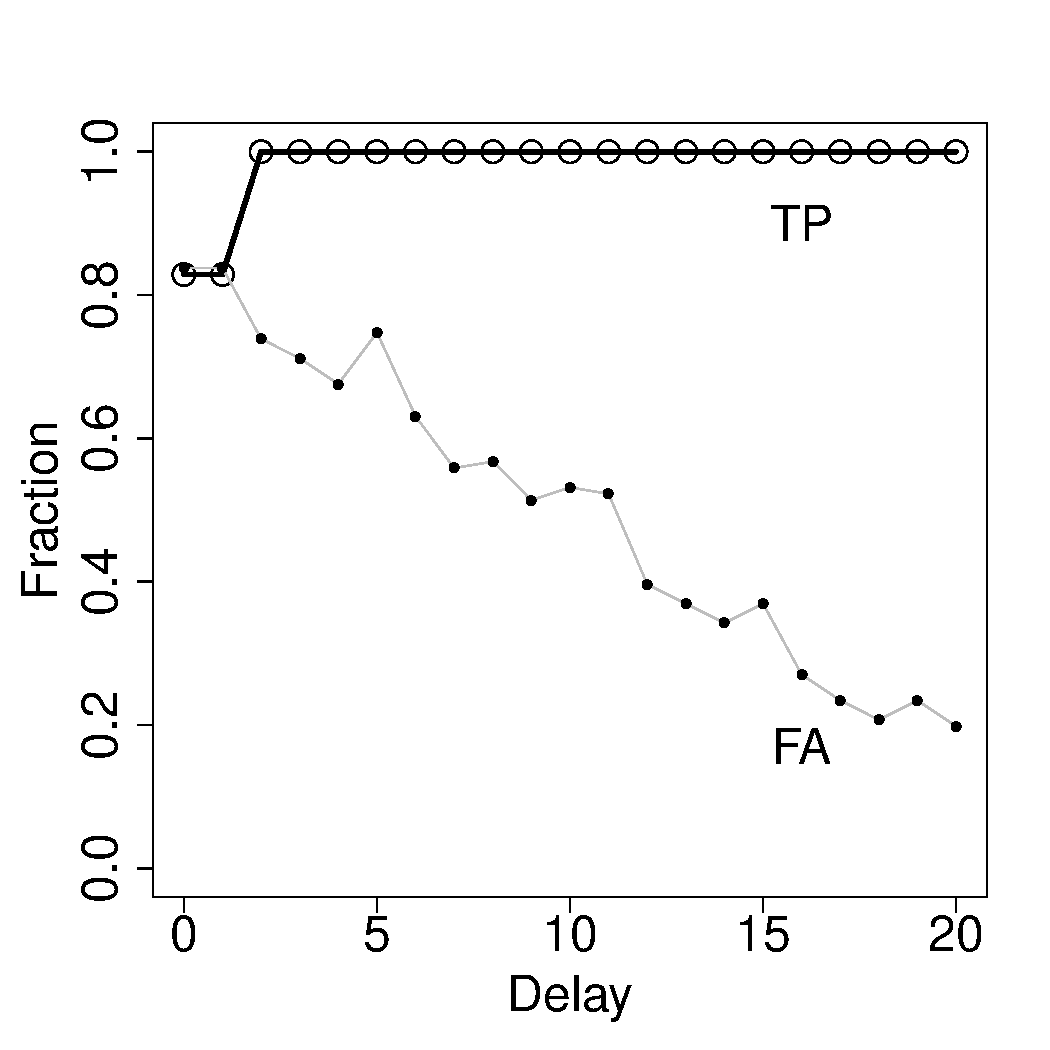
\includegraphics[ width=0.24\textwidth]{articles/pics/sdm_paper/performance2sdm.pdf}
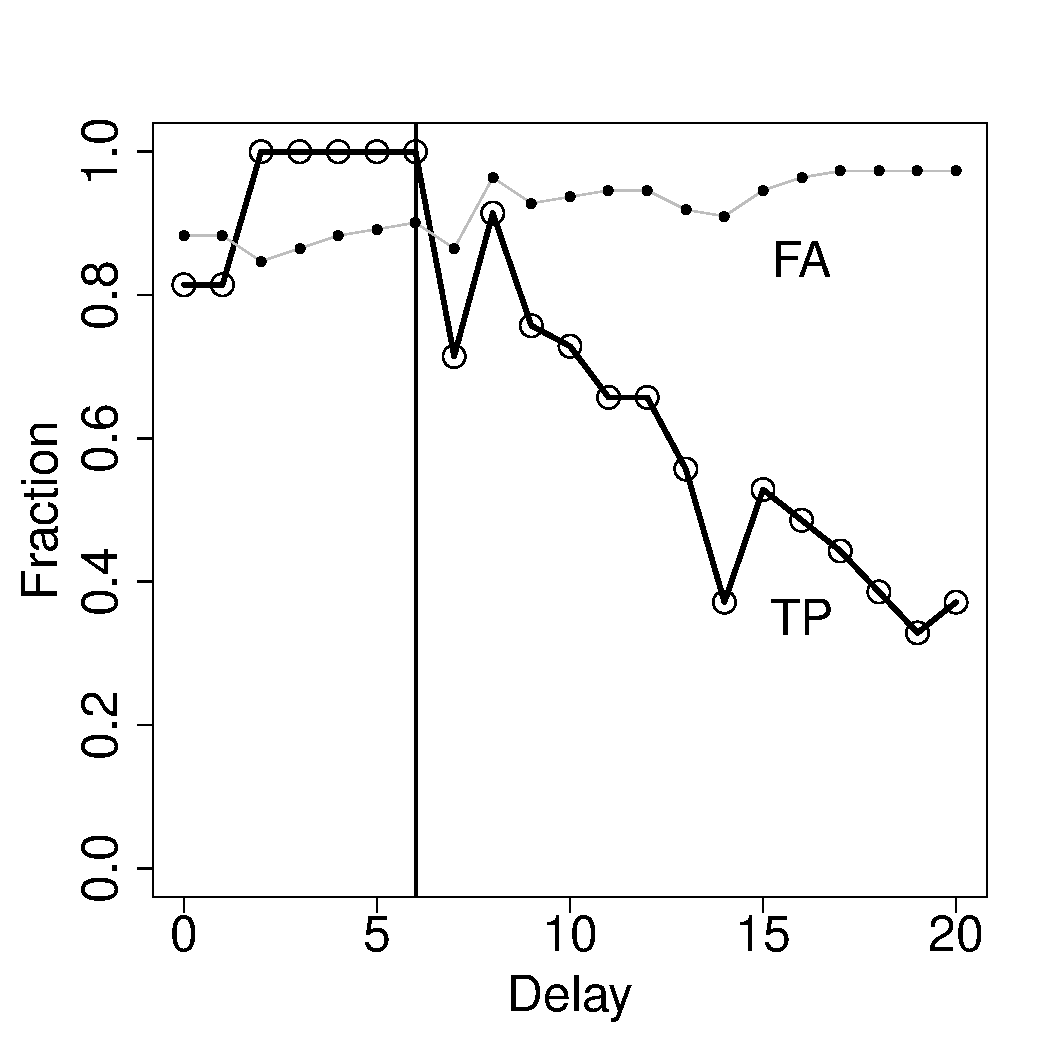
\includegraphics[ width=0.24\textwidth]{articles/pics/sdm_paper/performance1sdm.pdf}
\caption{
TP and FP rates of PCCF (not the base- or PCCF-enhanced detector) vs. the delay $D$ of change point confirmation.
}
\label{fig:combined}
\end{figure}

\subsection{Dynamic adjustment of sensitivity.}
This experiment demonstrates the pre-processing approach for integration of PCCF with a change detector, where detection sensitivity is adjusted online.
We first pre-calculate PCCF with parameters $\mu$ and $\sigma$, and then dynamically change the parameters according to the most recent probability of recurrent change.
Recall Figure~\ref{fig:naivedetector} depicting a toy example of dynamically changing threshold $h$ (dashed line).
When PCCF value is low, $h$ is set to a higher value $h_2$, when PCCF value is high, the detector threshold is set to $h_1$.

For this simulation we generate $200$ times input signal with $15$ recurrent changes and $15$ uniformly distributed outliers.
The average time interval between changes is $\mu = 10$ with the $\sigma = 0.5$.
The error rate is set to $\lambda = 1$, i.e.\ 1 outlier per time interval of width $\mu$.
To detect changes we used the same base-level detector as in the previous experiment.

The results are depicted in Figure~\ref{fig:rocdynamic}, showing TP and FP rates.
The performance of the detector without PCCF is depicted by the line with circles, obtained by varying the sensitivity threshold of the detector.
The performance of the detector with PCCF is depicted by the line with red squares, obtained by changing delay of the $c_i$ confirmation $D$ for a fixed threshold of the base detector.
We can see that performance of the detector can be improved using PCCF if $D < 2 \mu$.
This is in line with our theoretical results.
\begin{figure}[htb!]
\centering
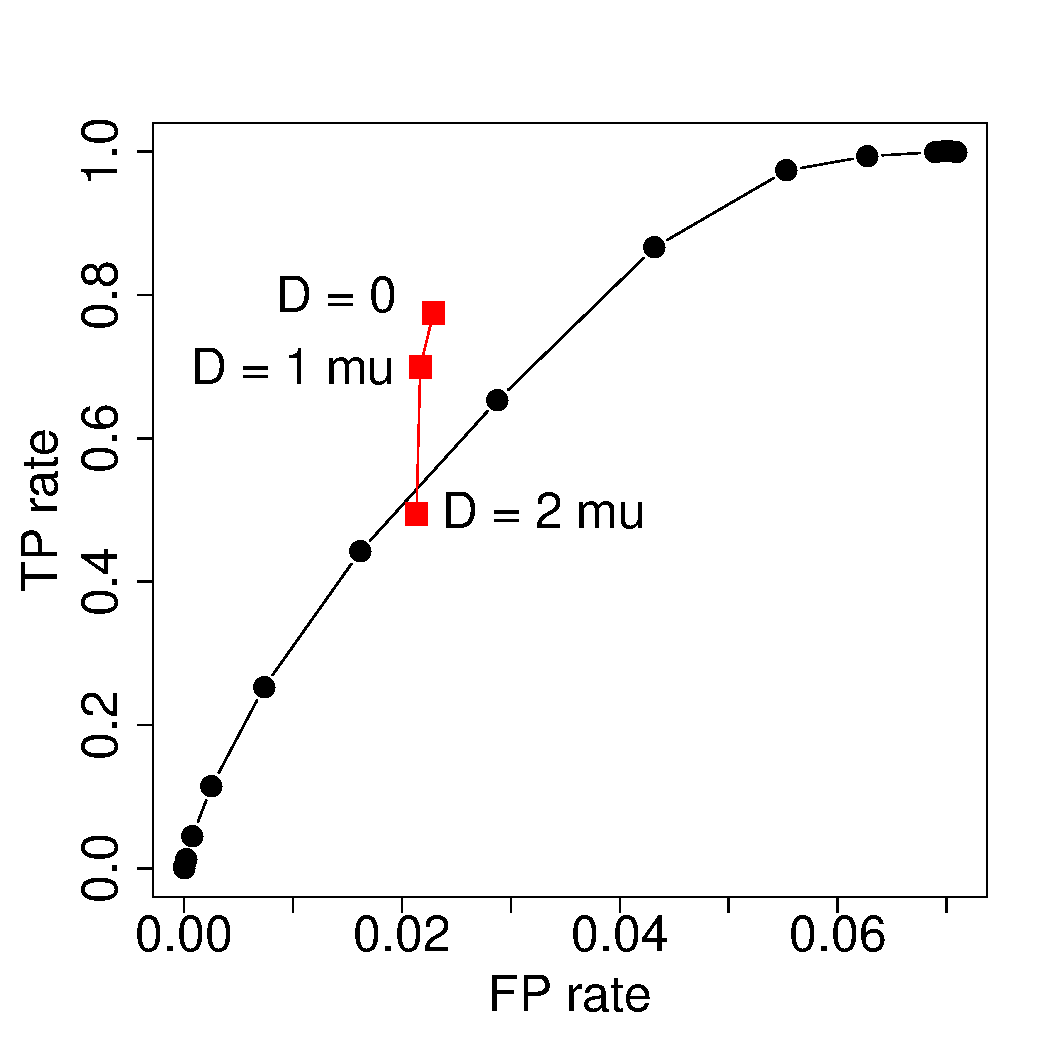
\includegraphics[width=0.30\textwidth]{articles/pics/sdm_paper/ROCImprovementAndDelay3}
\caption{
The trade-off between TPs and FPs.
Red squares show performance with the dynamic threshold with delayed feedback $(0, \mu, 2 \mu)$.}
\label{fig:rocdynamic}
\end{figure}

\subsection{Real datasets.} We experimented with two real datasets, the Boiler dataset that contains sensor readings containing recurrent refueling behavior, and the UK network traffic dataset with the typical recurrent aggregated traffic peaks.
\paragraph{Boiler dataset.}
Data comes from sensors installed on the scales measuring fuel mass in the container of Circulating Fluidized Bed boiler (CFB)~\cite{PechenizkiySIGKDDExpl09}.
The signal is shown in the top part of Figure~\ref{fig:cfbsig}, where the true changes are highlighted by vertical lines.
The mass of fuel decreases continuously as it is being consumed.
Abrupt changes in the signal happen at the start of the refueling process.
The signal is fluctuating due to rotating parts of the system making it difficult to distinguish the true changes from noise.

We calculated a series of PCCF,  updated after each provided confirmation with the delay $~ 2 \mu$ where $\mu$ is estimated from training data average distance between changes.
The results are shown in Figure~\ref{fig:cfbsig}.
PCCF functions are computed with confirmation delay $2\mu$ (bottom plot). Initial and updated PCCFs are marked by numbers.
Two outliers are correctly identified by PCCF and do not cause FPs.
%height = 0.35\textheight, width = 0.8\textwidth
\begin{figure}[htb!]
\centering
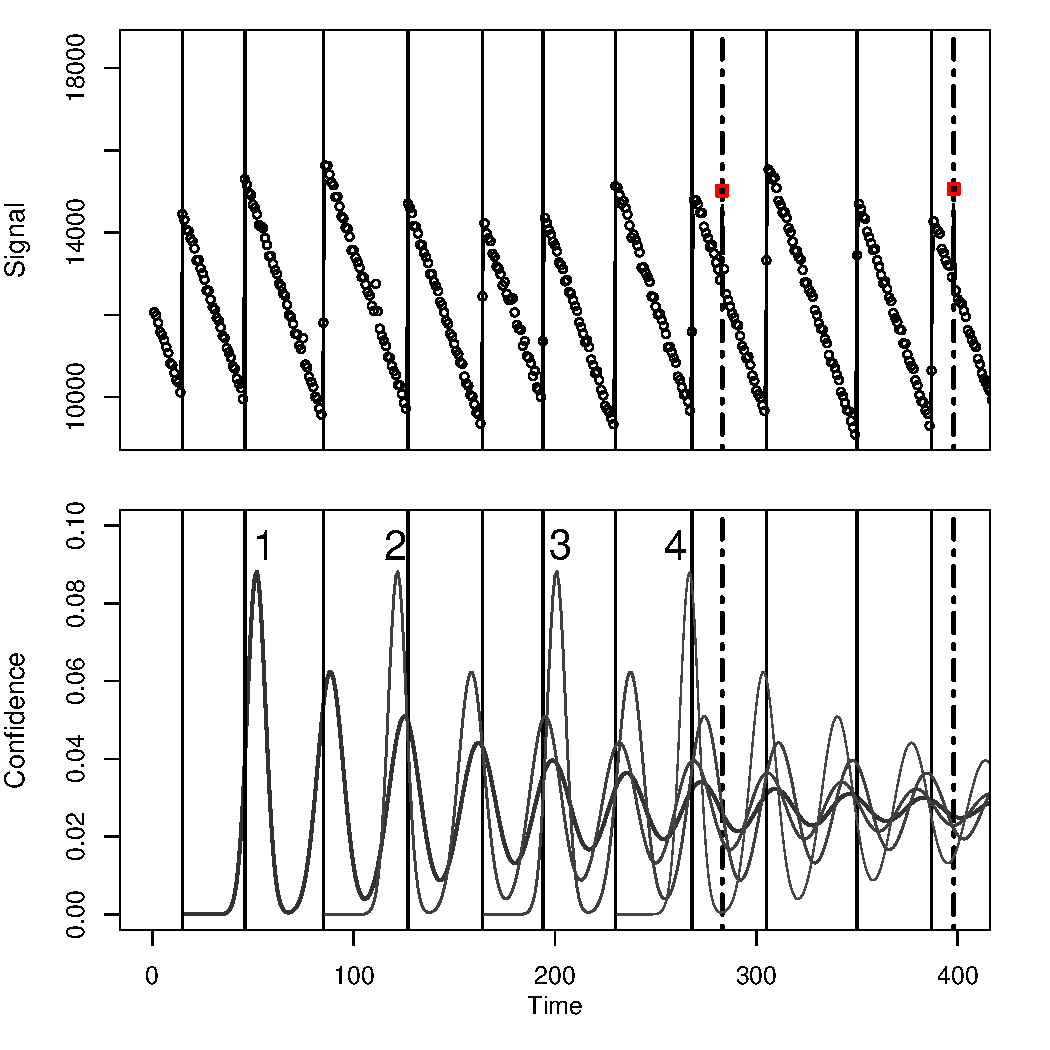
\includegraphics[width = 0.45\textwidth, height = 0.35\textheight, ]{articles/pics/sdm_paper/cfbproof2.pdf}
\caption{
The mass flow signal with abrupt changes (top) and updated PCCFs (bottom).
Outliers due to jammed particles (vertical dashed lines) in the mass flow do not result in FPs.
}
\label{fig:cfbsig}
\end{figure}

\paragraph{The Internet traffic dataset.}
Next, we test our approach on publicly available dataset\footnote{\url{https://datamarket.com/data/list/?q=internet+traffic+data+price\%3Afree}} containing aggregated internet traffic data from Internet Service Provider in the UK academic network backbone. The data series is illustrate in Figure~\ref{fig:trafficdata}.
%\href{https://datamarket.com/data/list/?q=internet+traffic+data+price\%3Afree}{https://datamarket.com/data/list/?q=internet+traffic+data+price\%3Afree}
%Data was collected between 19 November 2004
%, at 09:30 hours
%and 27 January 2005.
%, at 11:11 hours.
Measurements were taken between 19 Nov 2004 and 27 Jan 2005  at five minute intervals.
%Signal is visualized in Figure~\ref{fig:trafficdata}.
The task is to detect on-line maximum daily traffic by detecting changes in the trend of the signal.
These changes are periodic;  we do not use information of the daytime in order to consider them as recurrent.

Figure~\ref{fig:fractraffic} shows TP and FP rates of the PCCF-based detector for post-processing settings. The results are analogues for the results obtained in the experiment on the artificial data illustrated in Figure~\ref{fig:combined}. From the left plot we can see that max delay of confirmation is $D=6\mu$.

Figure~\ref{fig:rocdynamictraffic} illustrates improvement in the performance of the detector when using PCCF.
The ROC curve (solid line) shows the trade-off between TPs and FPs of the detector. %with fixed sensitivity threshold parameter.
Each point on this curve indicates the performance of the detector with a fixed sensitivity threshold.
The red triangles depict the performance of the PCCF-based detector with post-processing corresponding to the baseline `Static' detector (denoted with a blue diamond) we chose to improve as one already having a high TP rate but poor performance wrt FPs.
The red circles depict the performance of the PCCF-based detector with post-processing settings.
Different triangles and circles correspond to different values of $D$.
The triangles and circles concentrated in the top left corner with TP rate close to $1.0$ and FP rate close to $0$ correspond to setting when $D\leq6\mu$.
When $D>6\mu$ the triangles are drifting down showing the deterioration in the TP rate.
FP rate is not increasing because in both pre- and post-processing settings of PCCF-based detector we do not generate additions CDEs as we only reduced the sensitivity of a TP-optimal static detector we chose on the ROC.
\begin{figure}[htb!]
\centering
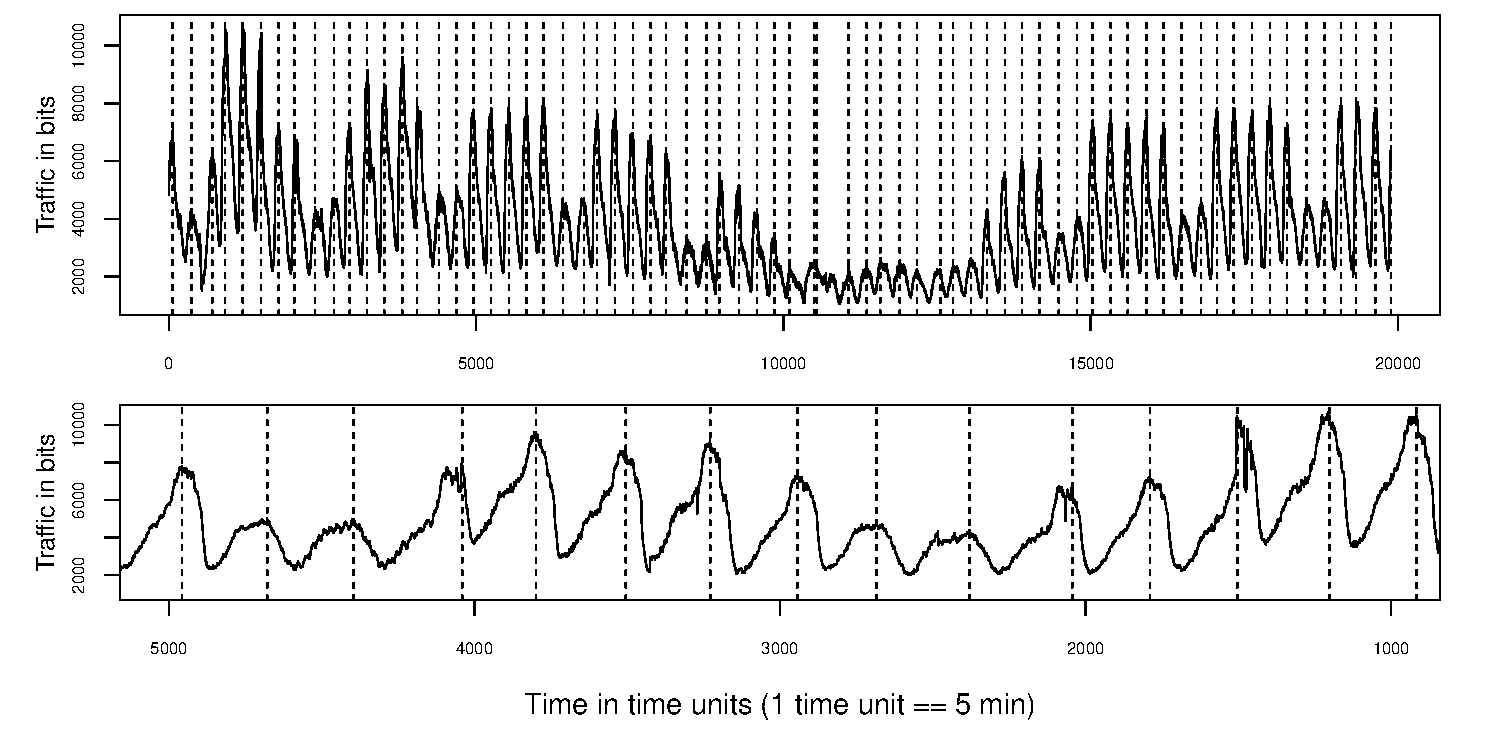
\includegraphics[width=0.48\textwidth]{articles/pics/sdm_paper/TrafficData.pdf}
\caption{
Aggregated traffic in the UK academic network.
The bottom figure in a zoomed region.
Dashed lines depict the true change points. % to be detected are depicted by vertical dashed lines.
}
\label{fig:trafficdata}
\end{figure}
%
\begin{figure}[htb!]
\centering
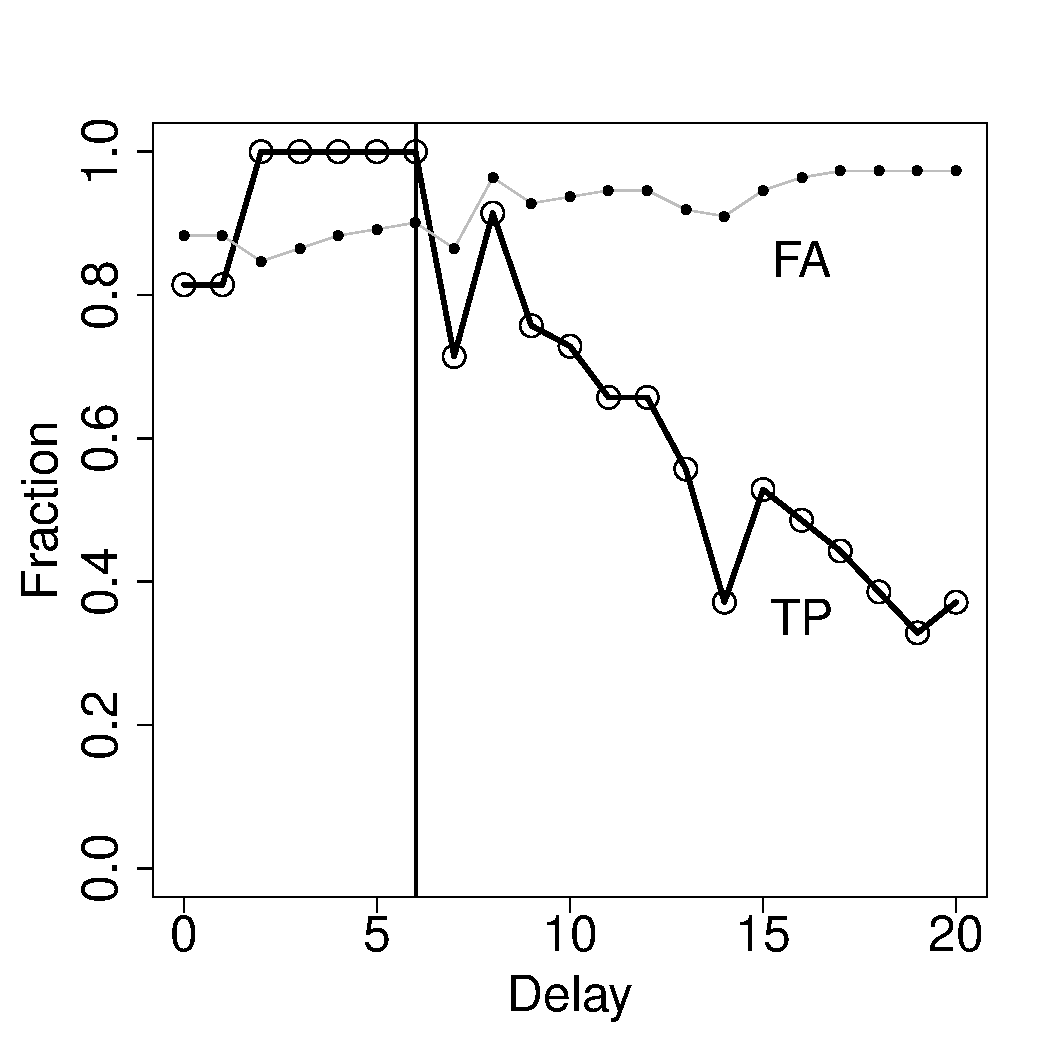
\includegraphics[width=0.24\textwidth]{articles/pics/sdm_paper/performance1sdm.pdf}
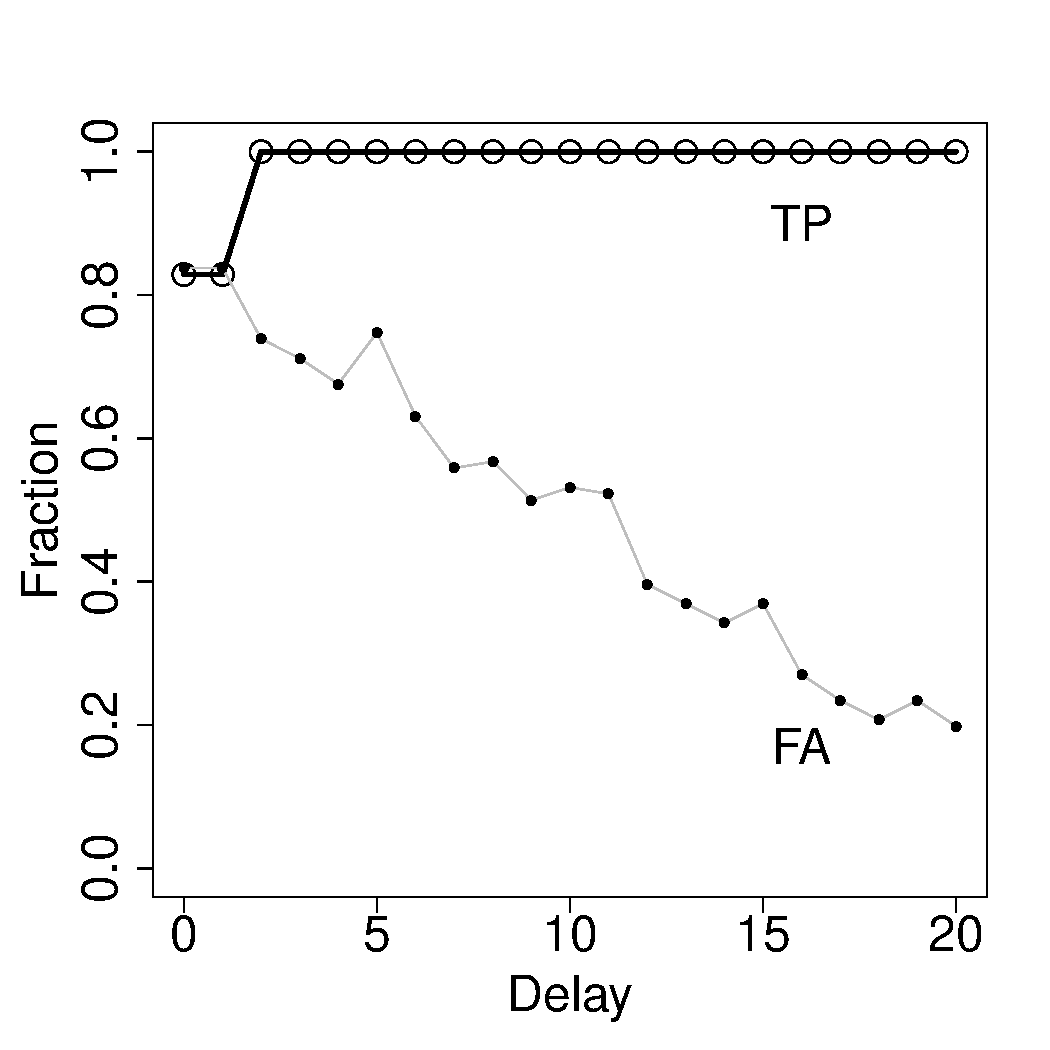
\includegraphics[width=0.24\textwidth]{articles/pics/sdm_paper/performance2sdm.pdf}
\caption{
PCCF sensitivity and specificity for the internet traffic dataset.
Threshold is higher (left) and lower (right) than PCCF limit.
The maximum delay of confirmation is $6 \mu $ (vertical line on the left plot).
}
\label{fig:fractraffic}
\end{figure}
%
\begin{figure}[htb!]
\centering
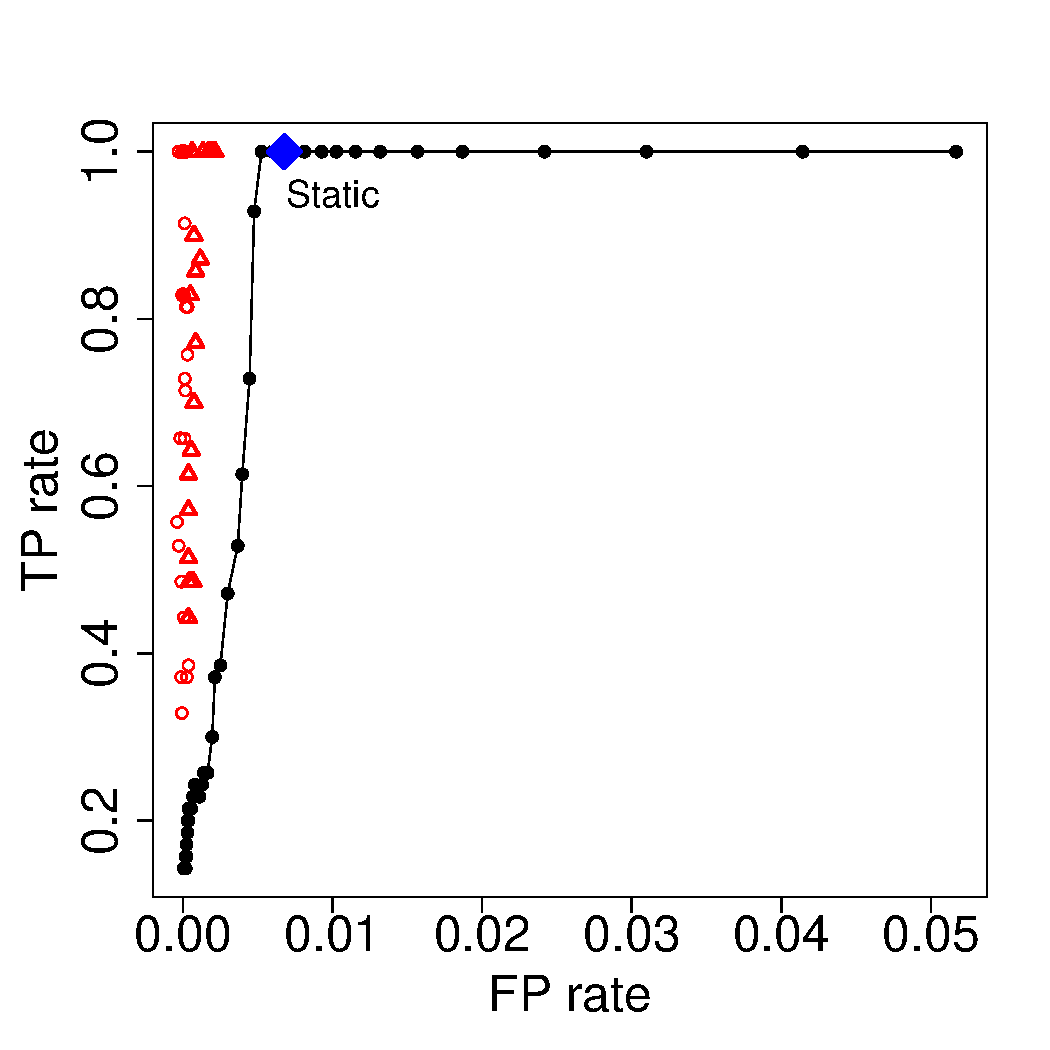
\includegraphics[width=0.3\textwidth]{articles/pics/sdm_paper/ROCimprtraff.pdf}
\caption{
	Black line - performance of the detector with static parameters.
	Red triangles - performance of PCCF based detector when applied to the  static detector with settings corresponding to the point marked as `Static'.
}
\label{fig:rocdynamictraffic}
\end{figure}

\subsection{Conclusions from experiments}
\label{subsec:conclusions}
For handling recurrent changes we introduced the predictive change confidence function (PCCF), which is a probability mass function, conditioned on the time of the last confirmed change.
We derived the performance guarantees analytically, assuming Gaussian distribution of the time intervals between changes, and verified the analytical expression for PCCF experimentally on synthetic data.
We proved that over time values of Gaussian PCCF converge to a limit value $L = \frac{1}{\mu}$ (Eq.~\ref{eq:pccf_limit_proof}).
%We presented two simple procedures for integrating PCCF with existing change detectors, and experimentally analyzed their performance.
We demonstrated on both synthetic and real datasets the feasibility of utilizing PCCF for recurrent change detection with two simple approaches: post-processing of manifested changes and dynamic adjustment of the sensitivity of the base-level detector.

The following conclusions can be made regarding the benefits of using recurrence information for improving detections' performance:
\begin{itemize}
  \item Recurrence information $\theta=(\mu, \sigma)$ is long-term useful if limit of the PCCF $L = \frac{1}{\mu}$ when $t \to \infty$ is greater than detector error rate $\frac{1}{\mu} > \lambda$ where $\mu$ is average time between recurrent changes.
  \item Recurrence information $\theta$ is short-term useful with the max confirmation delay $D$ if local maximums of the PCCF at moments $l \mu \leq D$ after confirmed change has higher values than probability of error $\lambda$,
      %$\mathcal{P}(t \leq D) > \lambda$
      but limit $L < \lambda$.
  %\item If $\sigma$ is `high' then PCCF converges very quickly to its limit $L$ and decision is made on the basis whether its value higher or lower than the error rate $\lambda$.
  %\item If $\sigma$ is `low' then PCCF oscillates during some time and usefulness is defined by whether values of the PCCF at the moments corresponding to the local maximums $k \mu$ are higher than $\lambda$ or not.
  \item The main factor defining usefulness of $\theta$ is the ratio $\frac{\mathcal{P}(t = l \mu)}{\lambda}$ within time $D$ from the most recently confirmed change and $\frac{L}{\lambda}$ in a longer term when we do not have confirmation or $D$ is high.
\end{itemize}
%Finally, we demonstrated on two real data sets that it is possible to improve change detection performance with the proposed approach.
In the performed experiments parameters $\theta$ were assumed to be known a priory or estimated from the training data.

This work provide several straightforward opportunities for future work, in particular investigating how uncertainty of $\theta$ estimates affects the performance of recurrent change detection, and studying other approaches for integrating PCCF with different existing change detection mechanisms.

\section{From BLPA: Integration with Bayesian detector}


\section{From Journal: Integration with CuSum}
